% Olympus v2 — system architecture (single-agent base + multi-agent overlay)
% Compile standalone:  pdflatex "architecture copy.tex"
% Same figure as architecture.tex, plus teal-dashed cards that mark the extra
% per-env workers (agents) which exist ONLY in the multi-agent case.
\documentclass[tikz,border=5pt]{standalone}
\usepackage{tikz}
\usepackage{amssymb}
\usepackage{helvet}
\renewcommand{\familydefault}{\sfdefault}
\usetikzlibrary{arrows.meta,positioning,fit,backgrounds}

\begin{document}
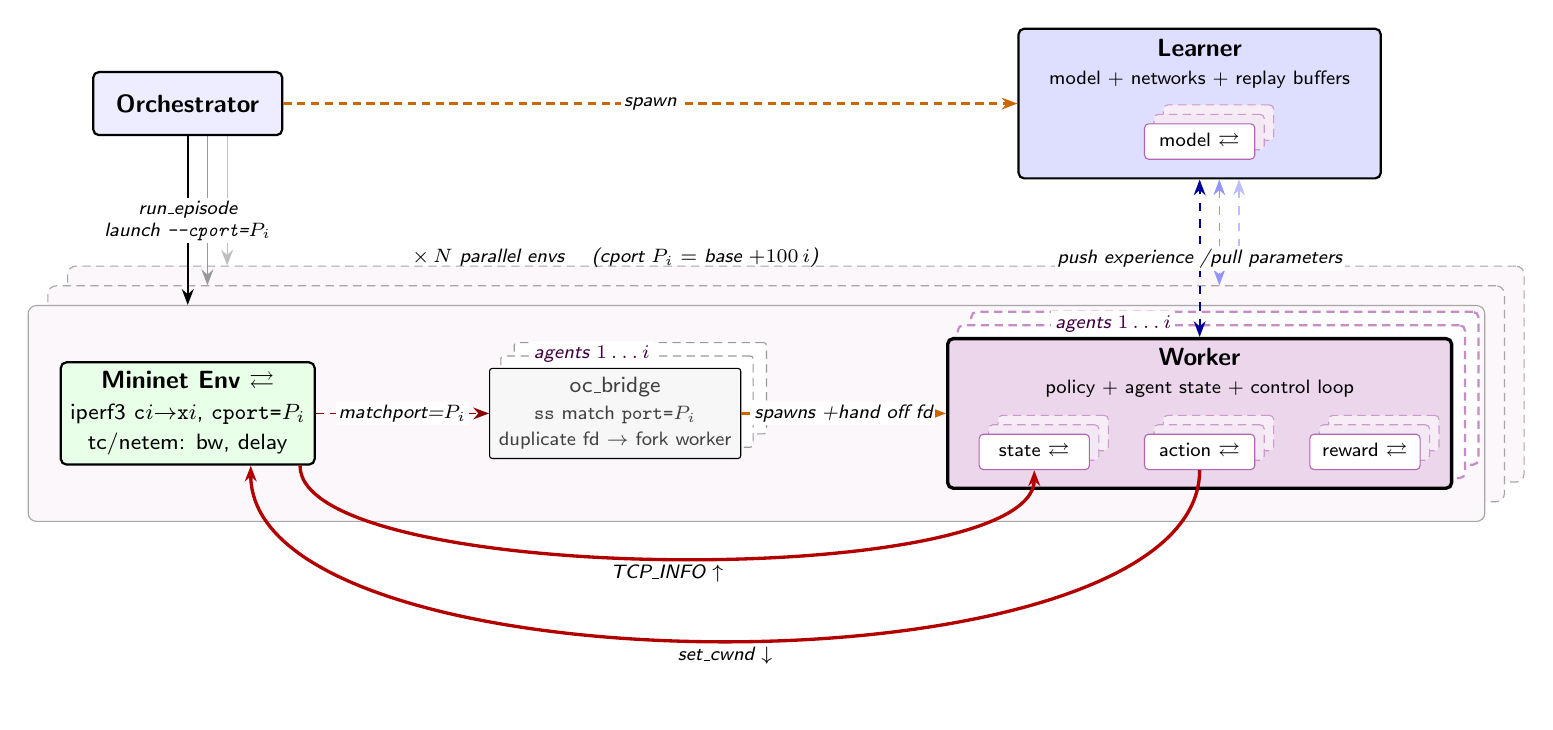
\begin{tikzpicture}[
  font=\small,
  node distance=14mm and 22mm,
  >={Stealth[length=2mm]},
  proc/.style={draw,rounded corners=2pt,thick,minimum height=8mm,
               minimum width=24mm,align=center,fill=blue!7},
  net/.style={draw,rounded corners=2pt,thick,minimum height=8mm,
              minimum width=30mm,align=center,fill=green!9},
  agent/.style={proc,fill=violet!16,very thick},
  bridge/.style={draw,solid,thin,rounded corners=1pt,
                 minimum height=8mm,minimum width=24mm,align=center,
                 fill=black!3,text=black!75,font=\footnotesize},
  card/.style={draw,rounded corners=3pt,thin,draw=black!35,fill=violet!3},
  ghostcard/.style={draw,densely dashed,rounded corners=3pt,thin,
                    draw=black!35,fill=violet!3},
  subbox/.style={draw,rounded corners=1.5pt,thin,draw=violet!60,fill=white,
                 font=\scriptsize,inner sep=2pt,
                 minimum width=14mm,minimum height=4.5mm},
  subbg/.style={draw,densely dashed,rounded corners=1.5pt,thin,
                draw=violet!40,fill=white,
                font=\scriptsize,inner sep=2pt,
                minimum width=14mm,minimum height=4.5mm},
  maonly/.style={draw=violet!45,densely dashed,thick,rounded corners=2pt,
                 fill=violet!7},
  listenercard/.style={draw=black!40,densely dashed,thin,rounded corners=1pt,
                       fill=white},
  agentcard/.style={draw=black!40,densely dashed,thin,rounded corners=2pt,
                    fill=white},
  ctrl/.style={->,thick},
  data/.style={->,very thick,draw=red!70!black},
  tap/.style={->,thin,draw=red!55!black,densely dashed},
  ipc/.style={<->,thick,draw=blue!60!black,dashed},
  cfg/.style={->,thick,draw=orange!80!black,densely dashed},
  lbl/.style={font=\scriptsize\itshape,fill=white,inner sep=1pt},
]

% ---- one rollout (= instance i): env --bridge--> worker(state/action) ----
\node[net] (env)
     {\textbf{Mininet Env} $\rightleftarrows$\\\footnotesize iperf3 \texttt{c$i$}$\to$\texttt{x$i$}, \texttt{cport=$P_i$}\\\footnotesize tc/netem: bw, delay};

\node[bridge,right=of env] (listener)
     {oc\_bridge \\\scriptsize \texttt{ss} match \texttt{port=$P_i$}\\\scriptsize duplicate fd $\to$ fork worker};

% worker shell, with internal state + action module decks
\node[agent,right=26mm of listener,minimum width=64mm,minimum height=19mm] (worker) {};
\node[align=center,anchor=north,inner sep=0pt] at ([yshift=-1.4mm]worker.north)
     {\textbf{Worker}\\[-1pt]\scriptsize policy + agent state + control loop};

% three swappable module decks across the worker bottom: state | action | reward

% -- state
\node[subbg,anchor=south,fill=violet!7] at ([xshift=-18.6mm,yshift=4.9mm]worker.south) {};
\node[subbg,anchor=south,fill=violet!9] at ([xshift=-19.8mm,yshift=3.7mm]worker.south) {};
\node[subbox,anchor=south] at ([xshift=-21mm,yshift=2.5mm]worker.south) (wstate) {state $\rightleftarrows$};

% -- action
\node[subbg,anchor=south,fill=violet!7] at ([xshift=2.4mm,yshift=4.9mm]worker.south) {};
\node[subbg,anchor=south,fill=violet!9] at ([xshift=1.2mm,yshift=3.7mm]worker.south) {};
\node[subbox,anchor=south] at ([xshift=0mm,yshift=2.5mm]worker.south) (waction) {action $\rightleftarrows$};

% -- reward
\node[subbg,anchor=south,fill=violet!7] at ([xshift=23.4mm,yshift=4.9mm]worker.south) {};
\node[subbg,anchor=south,fill=violet!9] at ([xshift=22.2mm,yshift=3.7mm]worker.south) {};
\node[subbox,anchor=south] at ([xshift=21mm,yshift=2.5mm]worker.south) (wreward) {reward $\rightleftarrows$};

% ---- control plane on the row above ----
\node[proc,above=20mm of worker,fill=blue!13,minimum width=46mm,minimum height=19mm] (learner) {};
\node[align=center,anchor=north,inner sep=0pt] at ([yshift=-1.4mm]learner.north)
     {\textbf{Learner}\\[-1pt]\scriptsize model + networks + replay buffers};

% swappable model deck inside the learner
\node[subbg,anchor=south,fill=violet!7] at ([xshift=2.4mm,yshift=4.9mm]learner.south) {};
\node[subbg,anchor=south,fill=violet!9] at ([xshift=1.2mm,yshift=3.7mm]learner.south) {};
\node[subbox,anchor=south] at ([xshift=0mm,yshift=2.5mm]learner.south) (lmodel) {model $\rightleftarrows$};

\node[proc] (orch) at (env |- learner) {\textbf{Orchestrator}};

% ---- stack the rollout row into N parallel environments ----
\begin{scope}[on background layer]
  % rear wide boxes are dashed
  \node[ghostcard,fit=(env)(worker),inner sep=4mm,xshift=5mm,yshift=5mm]   (roll3) {};
  \node[ghostcard,fit=(env)(worker),inner sep=4mm,xshift=2.5mm,yshift=2.5mm] (roll2) {};

  % front wide box is solid
  \node[card,fit=(env)(worker),inner sep=4mm] (rollout) {};

  % faint fan-out onto the other stacked rollouts
  \coordinate (e1) at (rollout.north -| env);
  \coordinate (w1) at (rollout.north -| worker);

  \draw[->,thin,draw=black!40]
        ([xshift=2.5mm]orch.south) -- ([shift={(2.5mm,2.5mm)}]e1);

  \draw[->,thin,draw=black!25]
        ([xshift=5mm]orch.south) -- ([shift={(5mm,5mm)}]e1);

  \draw[<->,thin,dashed,draw=blue!42]
        ([xshift=2.5mm]learner.south) -- ([shift={(2.5mm,2.5mm)}]w1);

  \draw[<->,thin,dashed,draw=blue!26]
        ([xshift=5mm]learner.south) -- ([shift={(5mm,5mm)}]w1);
\end{scope}

\node[font=\scriptsize\itshape,inner sep=1pt]
      at ([yshift=6mm]rollout.north -| listener)
      {$\times\,N$ parallel envs \quad (cport $P_i=$ base $+100\,i$)};

% ---- extra workers agents — present ONLY in the multi-agent case ----
\begin{scope}[on background layer]
  \node[maonly,fit=(worker),inner sep=0mm,xshift=3.2mm,yshift=3.2mm,fill=white] (maWorkerB) {};
  \node[maonly,fit=(worker),inner sep=0mm,xshift=1.5mm,yshift=1.5mm,fill=white] (maWorkerA) {};
\end{scope}

% ---- extra listener hand-offs — present ONLY in the multi-agent case ----
\begin{scope}[on background layer]
  \node[listenercard,fit=(listener),inner sep=0mm,xshift=3.2mm,yshift=3.2mm] (maListenerB) {};
  \node[listenercard,fit=(listener),inner sep=0mm,xshift=1.5mm,yshift=1.5mm] (maListenerA) {};
\end{scope}


\node[font=\scriptsize\itshape,text=violet!50!black,anchor=east,fill=white,inner sep=1.5pt]
     at ([xshift=5mm,yshift=1.8mm]listener.north) {agents $1\ldots i$};

\node[font=\scriptsize\itshape,text=violet!50!black,anchor=east,fill=white,inner sep=1.5pt]
     at ([xshift=-3mm,yshift=1.7mm]worker.north) {agents $1\ldots i$};

% ===== edges =====
\draw[cfg] (orch) -- node[lbl]{spawn} (learner);

\draw[ctrl] (orch) --
      node[lbl,align=center]{run\_episode\\launch \texttt{-{}-cport=$P_i$}}
      (rollout.north -| env);

\draw[ipc] (worker) --
      node[lbl]{push experience /\\pull parameters}
      (learner);

% the bridge attaches to THIS env, then forks the worker
\draw[tap] (env) --
      node[lbl]{match\\port=$P_i$}
      (listener);

\draw[cfg] (listener) --
      node[lbl]{spawns +\\hand off fd}
      (worker);

% the control loop lives between the worker and its env socket
\draw[data,->] (waction.south) to[out=-90,in=-90,looseness=0.62]
      node[lbl,pos=.5,below=0.3mm]{set\_cwnd $\downarrow$}
      ([xshift=8mm]env.south);

\draw[data,->] ([xshift=-2mm]env.south east) to[out=-90,in=-90,looseness=0.42]
      node[lbl,pos=.5,below=0.3mm]{TCP\_INFO $\uparrow$}
      (wstate.south);

\end{tikzpicture}
\end{document}